% Networks graphs
\subsection{Networks/Graphs} \label{s:lit:graph_overview}

Networks, or graphs, are represented by a set of nodes (or vertices) and the connections between them, known as edges or links, as seen in \cref{fig:graphs_basic}. Graphs can be represented mathematically via matrices (and even lists), which allows for powerful and efficient analysis of the nodes and their connections. As explained in the introduction of the bladder cancer (\cref{s:lit:biology}), representing and understanding the relationships between elements is essential in molecular biology, where genes' roles are intertwined, and different links enable different pathways.

Traditional clustering analyses, such as hierarchical clustering, do not take in account these relationships, partly because they are often unknown, and because the computational models do not have that layer of information built-in. A key aspect of genetics is the interdependence between elements, which makes networks a suitable candidate for analysing molecular data, as covered in more depth in \cref{s:lit:nets_bio}. Co-expression networks are one approach to modelling such connections by computing the pairwise correlation of gene expression to determine the strength of connections; the research conducted in this field is presented in \cref{s:lit:co_net}.

\begin{figure}[!t]
  \centering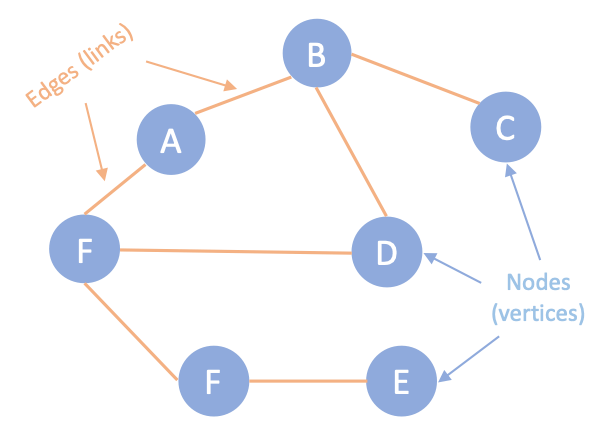
\includegraphics[width=0.6\textwidth,keepaspectratio]{Sections/Lit_review/Resources/basic_graphs.png}
    \caption[Basic graph]{Basic graphs illustrating gene interactions.}
    \label{fig:graphs_basic}
\end{figure}

% Weighted graphs
To model more complex relations between the genes and their interaction in the network, the edges are assigned weights values that either represent a strengthening or weakening in the links between nodes (genes). Data that can be tabulated and processed by various graph algorithms while the edges weights represent an opportunity to model the different data types available in the omics. The work on network integrative approaches in biological applications is covered in \cref{s:lit:net_data_int}.

% Finding nodes and community detections
A sub-field of graph theory and a crucial aspect of this project is finding community structures in a network. This means, how nodes can be grouped together based on their network properties, like the number of edges or connection strength. In the community detection research field clusters/groups/blocks and communities are used interchangeably, the preferred terms in this project are communities and blocks so that it is distinguishable from 'clusters' from cluster analysis methods like K-means. The two main school of thoughts, Modularity Maximisation and Stochastic Block Models, are extensively presented in \cref{s:lit:comm_detect} and used throughout the project, see \cref{s:N_I,s:N_I:sel_pruning,s:N_II}.


% The challenge with graphs is that they are less developed and can be computationally taxing. For example, community detection is a hot topic because there is no established method for identifying groups of nodes, and some popular methods can find patterns in noise. These issues are discussed at length in \cref{s:lit:comm_detect}.


\subsubsection*{Network metrics} \label{s:lit:net_metrics}

% Introduce the network metrics
In graph theory there are several methods to determine the role of the nodes into a network by considering different properties such as the number of edges, paths between the nodes, the strength of the connections, their centrality and others.

% node degree & PageRank
The node's degree represents the number of connections a node has, a higher number, the more important the node is to the network. There are several variations of the metric, counting only the edges inside or outside outside a community, the total number of connections as well as considering edges' weights. Throughout the project, the total degree is used.

% page rank
PageRank is a method that not only considers how many connections a node has but also takes the quality of these connections; i.e to which nodes it is connected. This method was first introduced by \citep{Brin1998-mc} and became the foundation of Google's search algorithm for ranking web pages. In a graph, PageRank assigns a score to each node based on the idea that a node is more important if it is linked to by other important nodes. This means that even if two nodes have the same number of connections (or degree), their PageRank scores can differ if one of them is connected to nodes with higher PageRank scores than the other. A vertex with higher PageRank value has a more important role in the network.

% closeness
There are three centrality metrics used in this project: closeness \citep{Opsahl2010-ok}, betweenness \citep{Freeman1977-qe}, and Katz centrality \citep{Katz1953-ie}. The first two metrics, closeness and betweenness, are employed to describe how close a node is to other nodes and how often it acts as an intermediary between them. Closeness centrality measures the average length of the shortest path from a node to all other nodes in the network; the shorter the distance, the more central the node is, meaning lower values indicate higher centrality. Betweenness centrality measures how often a node appears on the shortest path between two other nodes; higher values indicate that the node serves as a key connection point (or bridge) between other nodes. Katz centrality, the third metric, takes into account both the immediate neighbours of a node and their connections across the network. Higher values indicate that a node is important both locally and globally in the network, while lower values suggest a less influential role.

 
% IVI
In addition, the Integrated Value of Influence (IVI) \cite{Salavaty2020-wo} combines six different network metrics, including degree and betweenness centrality, as well as others like Neighbourhood Connectivity, which helps overcome the positional bias issue associated with betweenness centrality. The remaining three metrics—ClusterRank, local H-index, and Collective Influence—further complement the description of the network. The authors describe all six metrics and justify their use in their research \citet{Salavaty2020-wo}. The central idea of IVI is that it provides an integrated network score to account for both the local and global influence of a node within a network. Higher IVI values indicate that a node is more important at both local and global levels.


% Lower fence
The metrics are usually displayed in box plots as in \cref{fig:N_I:net_metrics_tum} with the points to show the different distribution in the values of the metrics. Using the box plots the outliers are marked by the lower, see \cref{eq:lower_fence},  and upper fence, see \cref{eq:higher_fence}, which are using the \acrfull{iqr} defined in \cref{eq:iqr}.

\begin{equation} \label{eq:lower_fence}
  \text{Lower Fence} = Q_1 - 1.5 \times \text{IQR}
\end{equation}

\begin{equation} \label{eq:higher_fence}
  \text{Upper Fence} = Q_3 + 1.5 \times \text{IQR}
\end{equation}

\begin{equation} \label{eq:iqr}
  \text{IQR} = Q_3 - Q_1
\end{equation}


\subsubsection*{Software used} \label{s:lit:net_software}

All the scores presented in this section are used to describe and understand the various networks generated throughout the project; see \cref{fig:N_I:net_metrics_p0,fig:N_I:net_metrics_tum} from \cref{s:N_I} and \cref{fig:N_II:net_metrics_comp,fig:N_II:net_metric_sig_std} from \cref{s:N_II}. 

In the first network chapter, \cref{s:N_I}, the Python version of iGraph \citep{Csardi2006-ez} is used to build the network, but it does not support the Katz centrality measure. However, in the second chapter, \cref{s:N_II}, and in the work on the Stochastic Block Model in \cref{s:N_I:sel_pruning}, the graph-tool Python package \citep{Peixoto2014-ls} is used, which supports Katz centrality.

